\documentclass[fleqn]{beamer}

\usetheme{Rochester}
\setbeamertemplate{navigation symbols}{}

\usepackage[style=alphabetic,maxalphanames=6]{biblatex}
\bibliography{quantitative}

\usepackage{amsmath}
\usepackage{amssymb}
\usepackage{cmll}
\usepackage{ebproof}
\usepackage{ebproof-rules}
\usepackage{mathpartir}
\usepackage{mathrsfs}
\usepackage{mathtools}
%\usepackage{natbib}
\usepackage{todonotes}
\usepackage{turnstile}

\usepackage{tikz}
\usetikzlibrary{tikzmark,fit}

\definecolor{use}{HTML}{008000}
\newcommand\gr[1]{{\color{use}#1}}
\newcommand\grctx[1]{\gr{\mathcal{#1}}}
\newcommand\grP{\grctx P}
\newcommand\grQ{\grctx Q}
\newcommand\grR{\grctx R}
\newcommand\grPprime{\grP\gr'}
\newcommand\grQprime{\grQ\gr'}
\newcommand\name{\ensuremath{\lambda\grR}}
\newcommand\grctxsub[2]{\grctx{#1}_{\gr{#2}}}
\newcommand\grPe{\grctxsub P e}
\newcommand\grPf{\grctxsub P f}
\newcommand\grQe{\grctxsub Q e}
\newcommand\grQf{\grctxsub Q f}
\newcommand\sem[1]{\left\llbracket{#1}\right\rrbracket}
\newcommand\size[1]{\left\lvert{#1}\right\rvert}
\newcommand\ps{\mathit{ps}}
\newcommand\qs{\mathit{qs}}
\newcommand\rs{\mathit{rs}}
\newcommand\dotto{\mathrel{\dot\to}}
\newcommand\dottimes{\mathbin{\dot\times}}
\newcommand\wand{\mathrel{\mathord{-}\hspace{-0.75ex}*}}
\newcommand\sep{\mathbin{*}}
\newcommand\env[1]{(#1\mathrm{-Env})}
\newcommand\thinningN{\mathrm{Thinning}}
\newcommand\thinning[2]{\thinningN~#1~#2}
\newcommand\V{\mathcal V}
\newcommand\C{\mathcal C}
\newcommand\sqin{\mathrel{\mathrlap{\sqsubset}{\mathord{-}}}}
\newcommand\sqni{\mathrel{\mathrlap{\sqsupset}{\mathord{-}}}}
\newcommand\subres{=}
\newcommand\Ann{\mathscr R}

\renewcommand\land{~\wedge~}
\renewcommand\lor{~\vee~}

\DeclareMathOperator\obj{Obj}
\let\hom\relax
\DeclareMathOperator\hom{Hom}
\DeclareMathOperator\id{id}
\DeclareMathOperator\sub{Sub}


\newcommand\Rel{\mathrm{Rel}}

\title{Beyond semirings?}
\author{James Wood}
\institute{University of Strathclyde \and Huawei Technologies R\&D UK}
\date{Meeting on Graded Types, 17th June 2022}

\begin{document}

\frame{\titlepage}

\begin{frame}{Introduction}
  \begin{itemize}
    \item Why semirings?
      \begin{itemize}
        \item Addition $\sim$ accumulation
        \item Multiplication $\sim$ modality
        \item Plenty of specific examples in the literature
      \end{itemize}
      \pause
    \item Why not semirings?
      \begin{itemize}
        \item Sometimes we don't have modalities, e.g MALL.
        \item Multiplication by zero ($\Box_0$) can act strangely.
        \item Functions are backwards to checking fragments in interactive
          programming with holes.
      \end{itemize}
  \end{itemize}
\end{frame}

\begin{frame}{Monoidal categories}
  \begin{columns}
    \pause
    \begin{column}{.455\linewidth}
      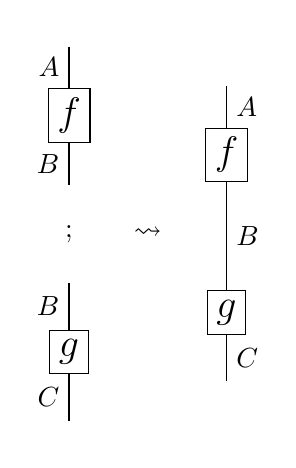
\begin{tikzpicture}[baseline]
        \path
        (-1,2.5) node(x) {}
        (-1,1.5) node[draw,rectangle](f) {\Large $f$}
        (-1,0.5) node(fx) {}
        ;
        \draw (x) -- node[left] {$A$} (f);
        \draw (f) -- node[left] {$B$} (fx);

        \node at (-1,0) {$;$};

        \path
        (-1,-0.5) node(y) {}
        (-1,-1.5) node[draw,rectangle](g) {\Large $g$}
        (-1,-2.5) node(gy) {}
        ;
        \draw (y) -- node[left] {$B$} (g);
        \draw (g) -- node[left] {$C$} (gy);

        \node at (0,0) {$\rightsquigarrow$};

        \path
        (1,2) node(x') {}
        (1,1) node[draw,rectangle](f') {\Large $f$}
        (1,-1) node[draw,rectangle](g') {\Large $g$}
        (1,-2) node(gfx') {}
        ;
        \draw (x') -- node[right] {$A$} (f');
        \draw (f') -- node[right] {$B$} (g');
        \draw (g') -- node[right] {$C$} (gfx');
      \end{tikzpicture}
    \end{column}
    \pause
    \begin{column}{.455\linewidth}
      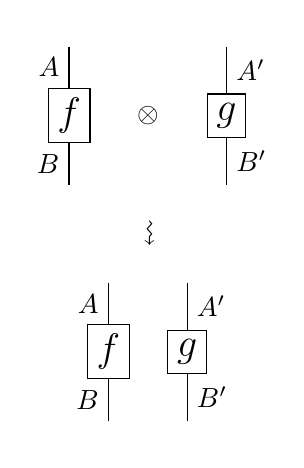
\begin{tikzpicture}[baseline]
        \path
        (-1,2.5) node(x) {}
        (-1,1.5) node[draw,rectangle](f) {\Large $f$}
        (-1,0.5) node(fx) {}
        ;
        \draw (x) -- node[left] {$A$} (f);
        \draw (f) -- node[left] {$B$} (fx);

        \node at (0,1.5) {$\otimes$};

        \path
        (1,2.5) node(y) {}
        (1,1.5) node[draw,rectangle](g) {\Large $g$}
        (1,0.5) node(gy) {}
        ;
        \draw (y) -- node[right] {$A'$} (g);
        \draw (g) -- node[right] {$B'$} (gy);

        \node[rotate=270] at (0,0) {$\rightsquigarrow$};

        \path
        (-0.5,-0.5) node(x) {}
        (-0.5,-1.5) node[draw,rectangle](f) {\Large $f$}
        (-0.5,-2.5) node(fx) {}
        ;
        \draw (x) -- node[left] {$A$} (f);
        \draw (f) -- node[left] {$B$} (fx);

        \path
        (0.5,-0.5) node(y) {}
        (0.5,-1.5) node[draw,rectangle](g) {\Large $g$}
        (0.5,-2.5) node(gy) {}
        ;
        \draw (y) -- node[right] {$A'$} (g);
        \draw (g) -- node[right] {$B'$} (gy);
      \end{tikzpicture}
    \end{column}
  \end{columns}
\end{frame}

\begin{frame}{Examples of monoidal categories}
  Examples of $(\mathcal C, I, \otimes)$:
  \begin{itemize}
    \item $(\Set, 1, \times)$ --- Cartesian structure of $Set$
    \item $(\Rel, 1, \times)$ --- \emph{Not} the Cartesian structure of $\Rel$
    \item $(\mathrm{CMon}, \mathbb N, \otimes_{\mathbb N})$ ---
      commutative monoids under their tensor product
    \item $(\Set_{\mathrm{part}}, 1, \times)$
  \end{itemize}
\end{frame}

\begin{frame}{Monoids in a monoidal category (identity)}
  \[
    \begin{tikzpicture}[baseline]
      \path
      (-3.5,1) node(0l) {0}
      (-1.5,2) node(xl) {}
      (-2.5,0) node(+l) {+}
      (-2.5,-1) node(resl) {}
      ;
      \path
      (-3.5,3) node {(0}
      (-2.5,3) node {+}
      (-1.5,3) node {x)}
      ;

      \draw (0l) -- (+l);
      \draw (xl) to[out=270,in=45] (+l);
      \draw (+l) -- (resl);

      \node at (-1,0) {=};
      \node at (-1,3) {=};

      \path
      (0,2) node(x) {}
      (0,-1) node(res) {}
      ;
      \path
      (0,3) node {x}
      ;

      \draw (x) -- (res);

      \node at (1,0) {=};
      \node at (1,3) {=};

      \path
      (3.5,1) node(0) {0}
      (1.5,2) node(x) {}
      (2.5,0) node(+) {+}
      (2.5,-1) node(res) {}
      ;
      \path
      (3.5,3) node {0)}
      (2.5,3) node {+}
      (1.5,3) node {(x}
      ;

      \draw (0) -- (+);
      \draw (x) to[out=270,in=135] (+);
      \draw (+) -- (res);
    \end{tikzpicture}
  \]
\end{frame}

\begin{frame}{Monoids in a monoidal category (associativity)}
  \[
    \begin{tikzpicture}[baseline]
      \path
      (-3,2) node(xl) {}
      (-2,2) node(yl) {}
      (-1,2) node(zl) {}
      (-2.5,1) node(x+y) {+}
      (-2,0) node(xy+z) {+}
      (-2,-1) node(resl) {}
      ;
      \path
      (-3,3) node {(x}
      (-2.5,3) node {+}
      (-2,3) node {y)}
      (-1.5,3) node {+}
      (-1,3) node {z}
      ;

      \draw (xl) to[out=270,in=135] (x+y);
      \draw (yl) to[out=270,in=45] (x+y);
      \draw (x+y) to[out=270,in=135] (xy+z);
      \draw (zl) to[out=270,in=45] (xy+z);
      \draw (xy+z) -- (resl);

      \path
      (0,0) node {=}
      (0,3) node {=}
      ;

      \path
      (3,2) node(zr) {}
      (2,2) node(yr) {}
      (1,2) node(xr) {}
      (2.5,1) node(y+z) {+}
      (2,0) node(x+yz) {+}
      (2,-1) node(resr) {}
      ;
      \path
      (3,3) node {z)}
      (2.5,3) node {+}
      (2,3) node {(y}
      (1.5,3) node {+}
      (1,3) node {x}
      ;

      \draw (zr) to[out=270,in=45] (y+z);
      \draw (yr) to[out=270,in=135] (y+z);
      \draw (y+z) to[out=270,in=45] (x+yz);
      \draw (xr) to[out=270,in=135] (x+yz);
      \draw (x+yz) -- (resr);
    \end{tikzpicture}
  \]
\end{frame}

\begin{frame}{Commutative monoids in a symmetric monoidal category}
  \[
    \begin{tikzpicture}[baseline]
      \path
      (-2,1) node(xl) {}
      (-1,1) node(yl) {}
      (-1.5,0) node(+l) {+}
      (-1.5,-1) node(resl) {}
      ;

      \draw (xl) to[out=270,in=135] (+l);
      \draw (yl) to[out=270,in=45] (+l);
      \draw (+l) to (resl);

      \node at (0,0) {=};

      \path
      (2,1) node(xr) {}
      (1,1) node(yr) {}
      (1.5,0) node(+r) {+}
      (1.5,-1) node(resr) {}
      ;

      \draw (xr) to[out=270,in=135] (+r);
      \draw (yr) to[out=270,in=45] (+r);
      \draw (+r) to (resr);
    \end{tikzpicture}
  \]
\end{frame}

\begin{frame}{Semirings in a monoidal category}
  Annihilation requires deletion, and distributivity requires duplication
  $\sim$ Cartesian category.
  \[
    \begin{tikzpicture}[baseline]
      \path
      (-3.5,1) node(0l) {0}
      (-1.5,2) node(xl) {}
      (-2.5,0) node(*l) {*}
      (-2.5,-1) node(resl) {}
      ;
      \path
      (-3.5,3) node {(0}
      (-2.5,3) node {*}
      (-1.5,3) node {x)}
      ;

      \draw (0l) -- (*l);
      \draw (xl) to[out=270,in=45] (*l);
      \draw (*l) -- (resl);

      \node at (-1,0) {=};
      \node at (-1,3) {=};

      \path
      (0,0) node(0) {0}
      (0,2) node(x) {}
      (0,-1) node(res) {}
      (0,1) node[circle,draw](del) {}
      ;

      \draw (0) -- (res);
      \draw (x) -- (del);

      \node at (0,3) {0};

      \node at (1,0) {=};
      \node at (1,3) {=};

      \path
      (3.5,1) node(0) {0}
      (1.5,2) node(x) {}
      (2.5,0) node(*) {*}
      (2.5,-1) node(res) {}
      ;
      \path
      (3.5,3) node {0)}
      (2.5,3) node {*}
      (1.5,3) node {(x}
      ;

      \draw (0) -- (*);
      \draw (x) to[out=270,in=135] (*);
      \draw (*) -- (res);
    \end{tikzpicture}
  \]
  Take the category of \emph{cocommutative comonoids} in our original monoidal
  category.
\end{frame}

\begin{frame}{There's no such thing as a partial semiring}
  Consider a comonoid
  $(M, \eta : M \rightharpoonup 1, \mu : M \rightharpoonup M \times M)$ in
  $\Set_{\mathrm{part}}$.

  We have:
  \[
    \begin{tikzpicture}[baseline]
      \path
      (-3.5,-1) node[circle,draw](0l) {}
      (-1.5,-2) node(xl) {z}
      (-2.5,0) node[circle,draw](+l) {}
      (-2.5,1) node(resl) {x}
      ;

      \draw (0l) -- (+l);
      \draw (xl) to[out=90,in=325] (+l);
      \draw (+l) -- (resl);

      \node at (-1,0) {=};

      \path
      (0,-2) node(x) {x}
      (0,1) node(res) {x}
      ;

      \draw (x) -- (res);

      \node at (1,0) {=};

      \path
      (3.5,-1) node[circle,draw](0) {}
      (1.5,-2) node(x) {y}
      (2.5,0) node[circle,draw](+) {}
      (2.5,1) node(res) {x}
      ;

      \draw (0) -- (+);
      \draw (x) to[out=90,in=225] (+);
      \draw (+) -- (res);
    \end{tikzpicture}
  \]

  By determinism of duplicate, we must have $\mathrm{dup}(x) = (x, x)$.

  Furthermore, we see that every $x$ is in the counit.
\end{frame}

\begin{frame}{What can we do?}
  \begin{itemize}
    \item Find a different category of partial functions.
    \item Modify multiplication to avoid general distributivity/annihilation.
  \end{itemize}
\end{frame}

\begin{frame}{$\Set_{\mathrm{part}}$ is strict}
  \begin{itemize}
    \item A \emph{generalised element} of $A$ is a morphism of type $I \to A$.
    \item Generalised elements of $\Set_{\mathrm{part}}$ include $\bot$, where
      $\bot({*})\uparrow$.
    \item $\Set_{\mathrm{part}}$ models \emph{strict} partial functions ---
      preserve $\bot$.
  \end{itemize}
\end{frame}

\begin{frame}{Non-strict partial functions}
  Inspired by domain theory:
  \begin{itemize}
    \item Impose an information ordering $\sqsubseteq$.
    \item Morphisms are monotone, but don't preserve $\bot$ element.
    \item E.g, $0 * \bot = 0$.
    \item In fact, the $\{0,1,\omega\}$ semiring works as-is ($\bot = \omega$).
      \pause
    \item Typing derivations should avoid $\bot$.
    \item How does the information ordering interact with subgrading?
  \end{itemize}
\end{frame}

\begin{frame}{Commutative monoid with actions}
  \begin{block}{Definition: monoid with actions}
    A commutative monoid $M$ together with a set of monoid endomorphisms
    (\emph{actions}) $A$ closed under identity and composition.
  \end{block}
  \only<1>{%
    Expanding that, we have, for any action $\rho$ and elements $x$ and $y$:
    \begin{itemize}
      \item $\rho(0) = 0$
      \item $\rho(x + y) = \rho(x) + \rho(y)$
    \end{itemize}
    Note that this is not the same as a module.
  }
  \only<2>{%
    \begin{block}{Example: linearity in $\Rel$}
      Let $M = (\{0,1,\omega\}, \{0,\omega\}, +)$, where:
      % \begin{itemize}
      %   \item $0 + 0 = 0$
      %   \item $0 + 1 = 1$
      %   \item $1 + 0 = 1$
      %   \item $\omega + \omega = \omega$
      % \end{itemize}
      % TODO: sort out indentation issues
      \begin{columns}
        \begin{column}{.455\linewidth}
          \begin{itemize}
            \item $0 + 1 = 1$
            \item $1 + 0 = 1$
          \end{itemize}
        \end{column}
        \begin{column}{.455\linewidth}
          \begin{itemize}
            \item $0 + 0 = 0$
            \item $\omega + \omega = \omega$
          \end{itemize}
        \end{column}
      \end{columns}
      \vspace{1ex}
      Let $A = \{1, \omega\}$, where:
      \begin{itemize}
        \item $1(x) = x$
        \item $\omega(x) = x$ when $x \neq 1$
      \end{itemize}
    \end{block}
  }
\end{frame}

%\begin{frame}{Many commutative monoids}
%  L/nL example with two modes (as in CMTT).
%
%  \[
%    \begin{tikzpicture}
%      \node(01) at (-1,0) {$\{0,1\}$};
%      \node(omega) at (1,0) {$\{0,\omega\}$};
%      \draw[->] (01) -- node[above] {$\omega$} (omega);
%    \end{tikzpicture}
%  \]
%\end{frame}

\begin{frame}{Conclusions}
  \begin{itemize}
    \item Sometimes we can't find the right semiring.
    \item There are several ways to weaken the definition of semiring.
    \item Which are worth exploring?
  \end{itemize}
\end{frame}

\end{document}
